% ****** Start of file apssamp.tex ******
%
%   This file is part of the APS files in the REVTeX 4.2 distribution.
%   Version 4.2a of REVTeX, December 2014
%
%   Copyright (c) 2014 The American Physical Society.
%
%   See the REVTeX 4 README file for restrictions and more information.
%
% TeX'ing this file requires that you have AMS-LaTeX 2.0 installed
% as well as the rest of the prerequisites for REVTeX 4.2
%
% See the REVTeX 4 README file
% It also requires running BibTeX. The commands are as follows:
%
%  1)  latex apssamp.tex
%  2)  bibtex apssamp
%  3)  latex apssamp.tex
%  4)  latex apssamp.tex
%
\documentclass[%
 reprint,
%superscriptaddress,
%groupedaddress,
%unsortedaddress,
%runinaddress,
%frontmatterverbose, 
%preprint,
%preprintnumbers,
%nofootinbib,
%nobibnotes,
%bibnotes,
 amsmath,amssymb,
 aps,
%pra,
%prb,
%rmp,
%prstab,
%prstper,
%floatfix,
]{revtex4-2}
\usepackage{tikz-cd}
\usepackage{subcaption}
\usepackage{graphicx}% Include figure files
\usepackage{dcolumn}% Align table columns on decimal point
\usepackage{float}
\usepackage{bm}% bold math
%\usepackage{hyperref}% add hypertext capabilities
%\usepackage[mathlines]{lineno}% Enable numbering of text and display math
%\linenumbers\relax % Commence numbering lines

%\usepackage[showframe,%Uncomment any one of the following lines to test 
%%scale=0.7, marginratio={1:1, 2:3}, ignoreall,% default settings
%%text={7in,10in},centering,
%%margin=1.5in,
%%total={6.5in,8.75in}, top=1.2in, left=0.9in, includefoot,
%%height=10in,a5paper,hmargin={3cm,0.8in},
%]{geometry}

\begin{document}

\preprint{APS/123-QED}

\title{Testing Clumping-Factor Estimators in the THESAN Simulations}% Force line breaks with \\

\author{Carlos Lopez Villanueva}
 \email{carlos.lopez-villanueva@polytechnique.edu}
\affiliation{%
 HEP Master, Institut Polytechnique de Paris
}%


\date{\today}% It is always \today, today,
             %  but any date may be explicitly specified

%\keywords{Suggested keywords}%Use showkeys class option if keyword
                              %display desired
\maketitle

%\tableofcontents
\section{Introduction}
This report compares the clumping-factor estimators proposed by Davies et al.~\cite{Davies_2026} and tests the assumptions underlying them using the THESAN simulations~\cite{Garaldi_2022}. The comparison is made against a direct, cell-based calculation of the clumping factor and against the intermediate quantities entering the approximate estimators.

We first describe the numerical calculation of the density field, mean free path, and photoionization rate. We then define the reference clumping factor and examine the assumptions used to derive the two approximate estimators considered here. Finally, we compare their predictions for different choices of the IGM mask.

\section{Methodology}
Our calculation proceeds in three steps. First, we construct the density field by assigning the gas-cell masses to the simulation cells. Second, we define an IGM mask using the overdensity and neutral-fraction cuts. Finally, we evaluate the required volume-weighted averages over the selected cells.

The main numerical choice concerns the representation of the density field. We can either use the Voronoi gas cells supplied with the simulation or construct a Cartesian grid and smooth particles whose spatial extent overlaps several grid cells. We use the Voronoi cells for the results presented below. Both approaches were tested; the Cartesian-grid calculation gives a systematically lower clumping factor, by up to 30\%, with the difference increasing towards higher redshift and for less restrictive IGM masks.

The approximate estimators additionally require the mean free path and the volume-weighted photoionization rate in ionized cells.

\subsection{Mean free path}
For the mean-free-path calculation, we use the random-origin, random-direction lines of sight provided with both THESAN-1 and THESAN-2.

We traverse each line of sight until the cumulative optical depth reaches unity. For each path element,
\begin{equation}
d\tau = \rho\,x_{\mathrm{HI}}\,\frac{X}{m_{\mathrm H}}\,\sigma_{912}\,dl,
\end{equation}

where $X=0.76$ is the hydrogen mass fraction and $\sigma_{912}=6.3\times10^{-18}\,\mathrm{cm^2}$. All quantities in this expression are evaluated in CGS units.

The distance at which $\tau=1$ defines the mean free path for that line of sight. We average these distances over the available lines of sight and convert the result to proper Mpc/$h$.

Repeating this procedure for every line of sight gives the simulation-wide mean free path for the chosen IGM mask.

\subsection{Photoionization rate}
For the photoionization rate, we use the Voronoi gas cells from the simulation and restrict the average to cells with $x_{\mathrm{HI}}<0.5$.

The publicly available THESAN snapshots provide the radiation field in three photon groups. The frequency integral therefore becomes

\begin{equation}
\Gamma_{\mathrm{HI}} = c\int_{\nu_0}^{\infty}n_\gamma(\nu)\sigma_{\mathrm{HI}}(\nu)\,d\nu
\simeq \sum_{b=1}^{3}n_{\gamma,b}\langle c\sigma_{\mathrm{HI}}\rangle_b.
\end{equation}

We use
\begin{equation}
\langle c\sigma_{\mathrm{HI}}\rangle_b =
\left(9.913\times10^{-8},\,2.095\times10^{-8},\,3.269\times10^{-9}\right)\,\mathrm{cm^3\,s^{-1}}.
\end{equation}

The photoionization rate is first computed for each cell and then volume-averaged over the selected cells.








\section{Reference clumping factor}

The direct calculation provides a reference against which the approximate estimators can be compared. The result depends on the adopted IGM definition, so we evaluate it as a function of the overdensity cutoff.

The definition used by Davies et al. is
$$ C \equiv \frac{\left\langle n_e n_{\mathrm{H\,II}} \alpha_{\mathrm{H\,II}} \right\rangle}
{\left\langle n_e \right\rangle
 \left\langle n_{\mathrm{H\,II}} \right\rangle
 \left\langle \alpha_{\mathrm{H\,II}} \right\rangle}.$$

We also evaluate the corresponding expression after restricting the calculation to ionized hydrogen. The resulting definitions are compared in Fig.~\ref{fig:clumping-factor-definitions}.

\begin{figure}[ht]
    \centering

    \begin{subfigure}{0.48\textwidth}
        \centering
        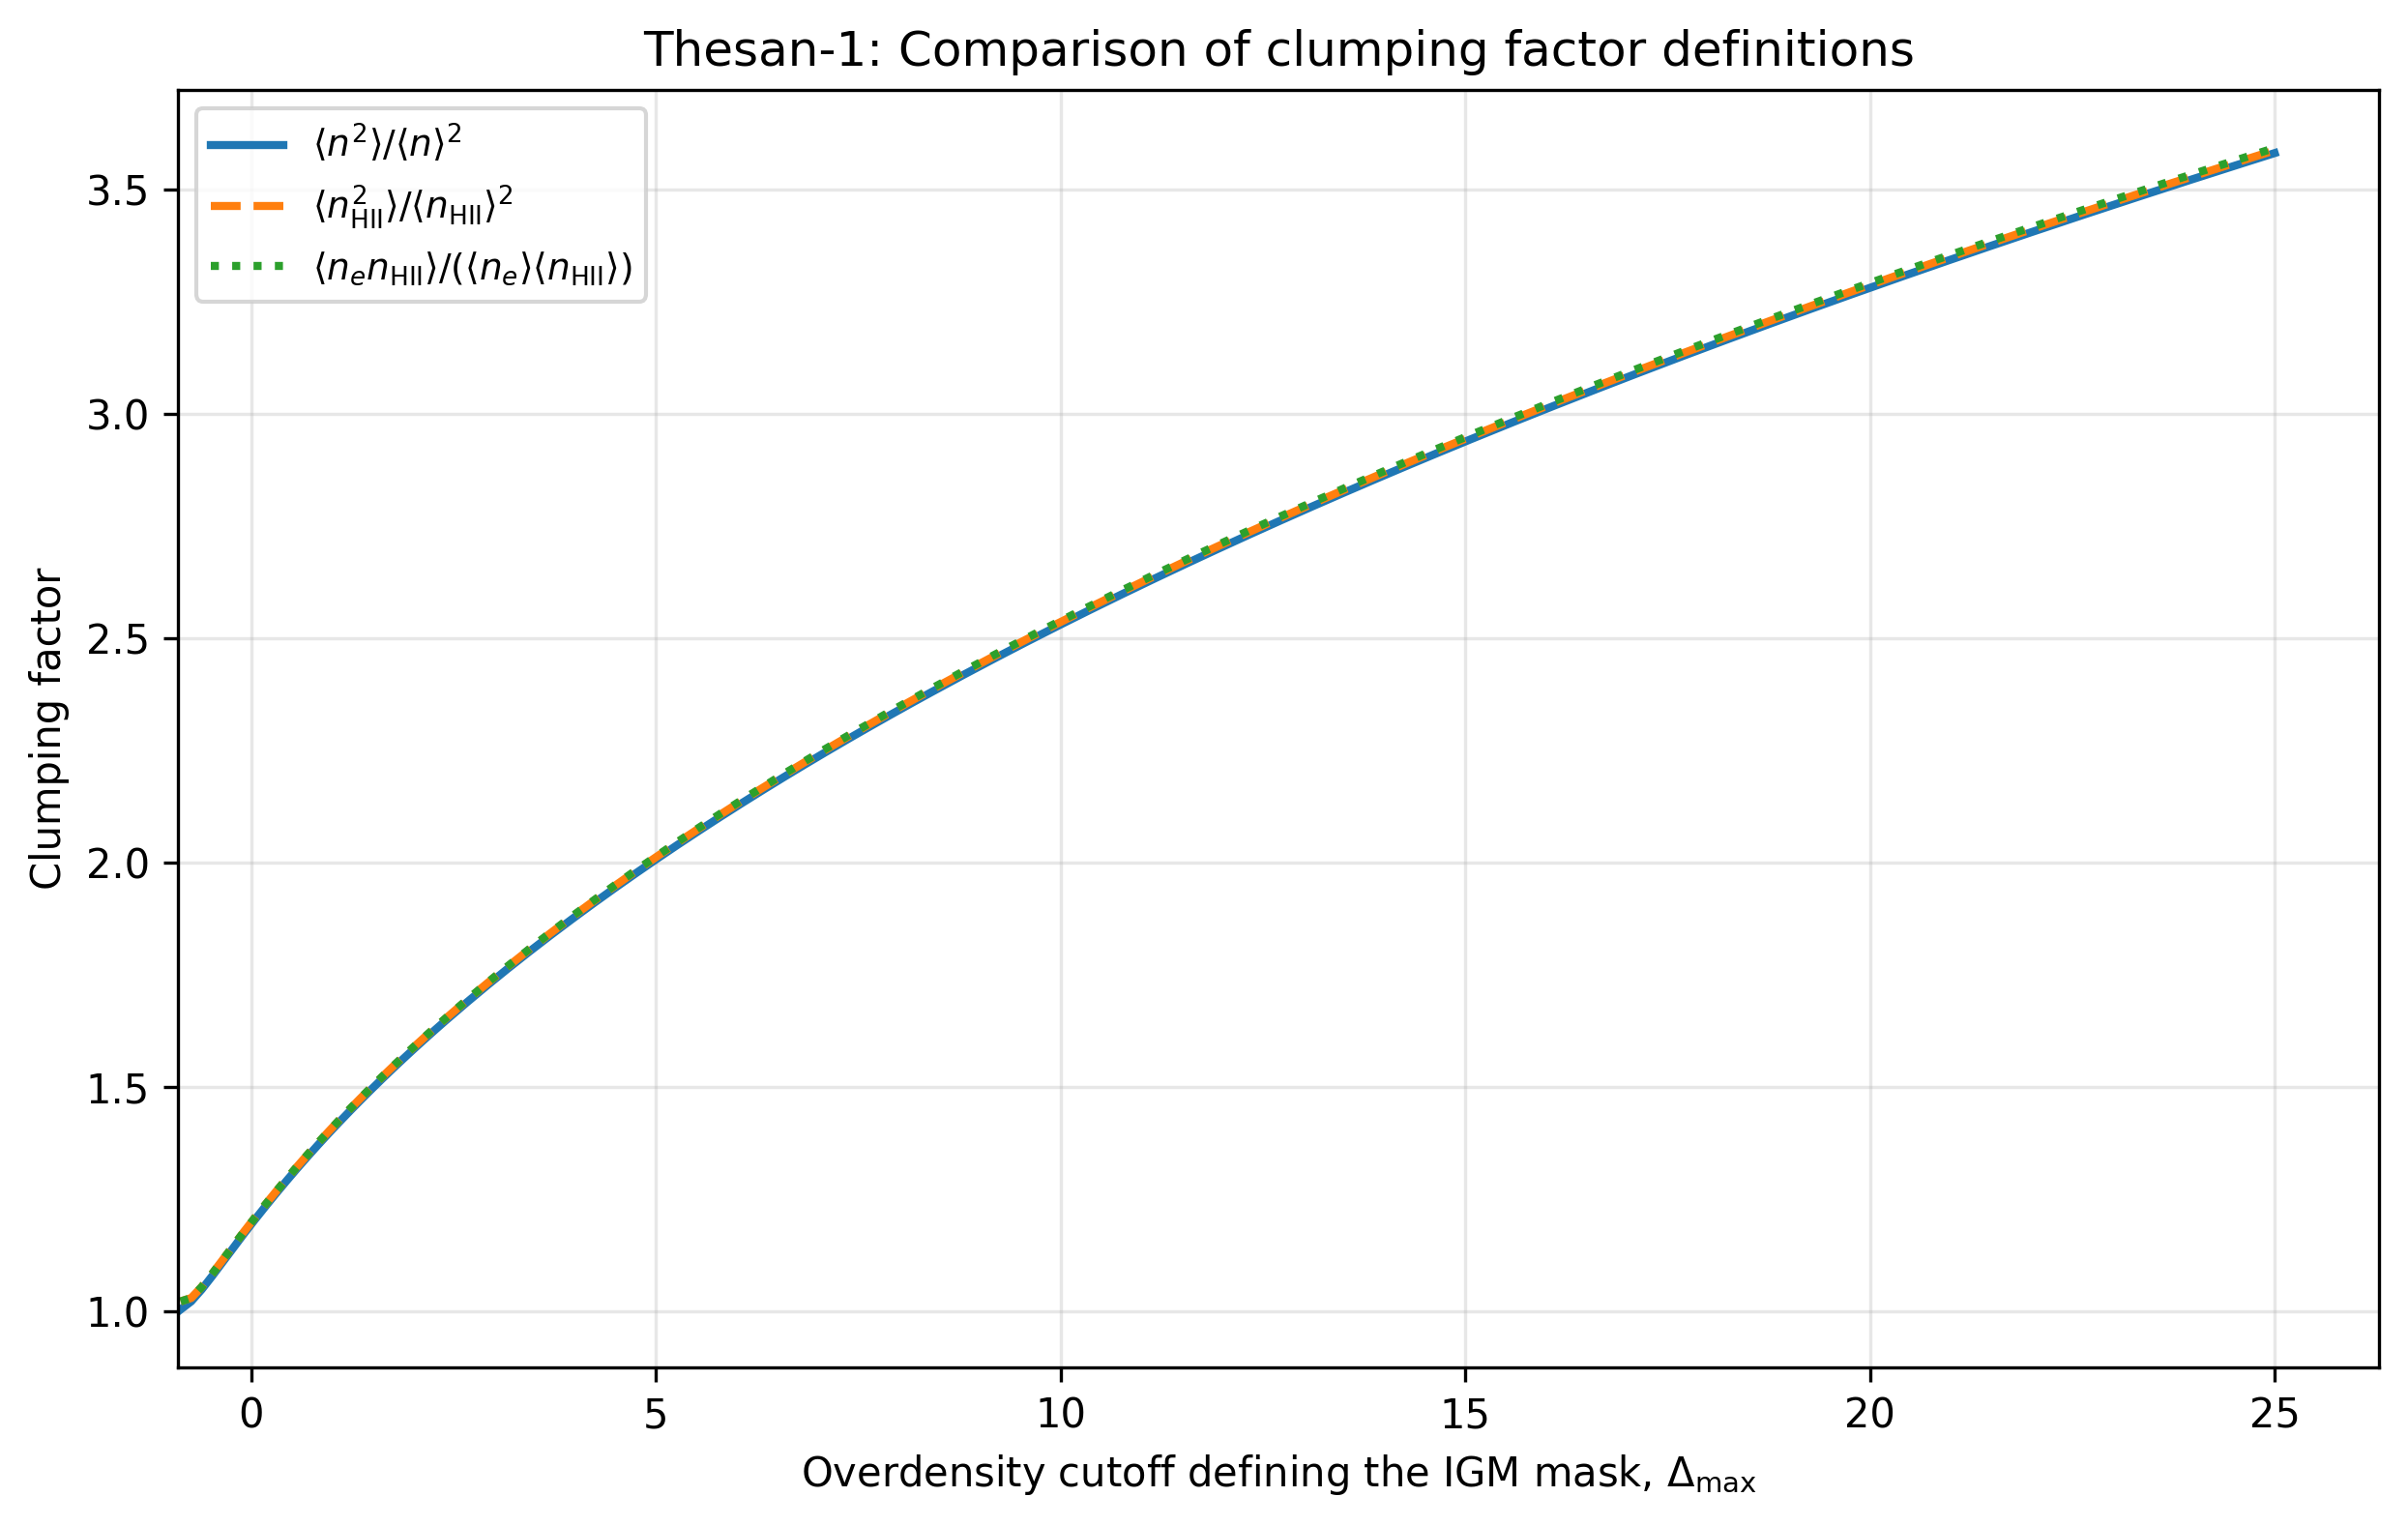
\includegraphics[width=\linewidth]{figures/thesan1_clumping_definitions_snapshot080.png}
    \end{subfigure}
    \hfill
    \begin{subfigure}{0.48\textwidth}
        \centering
        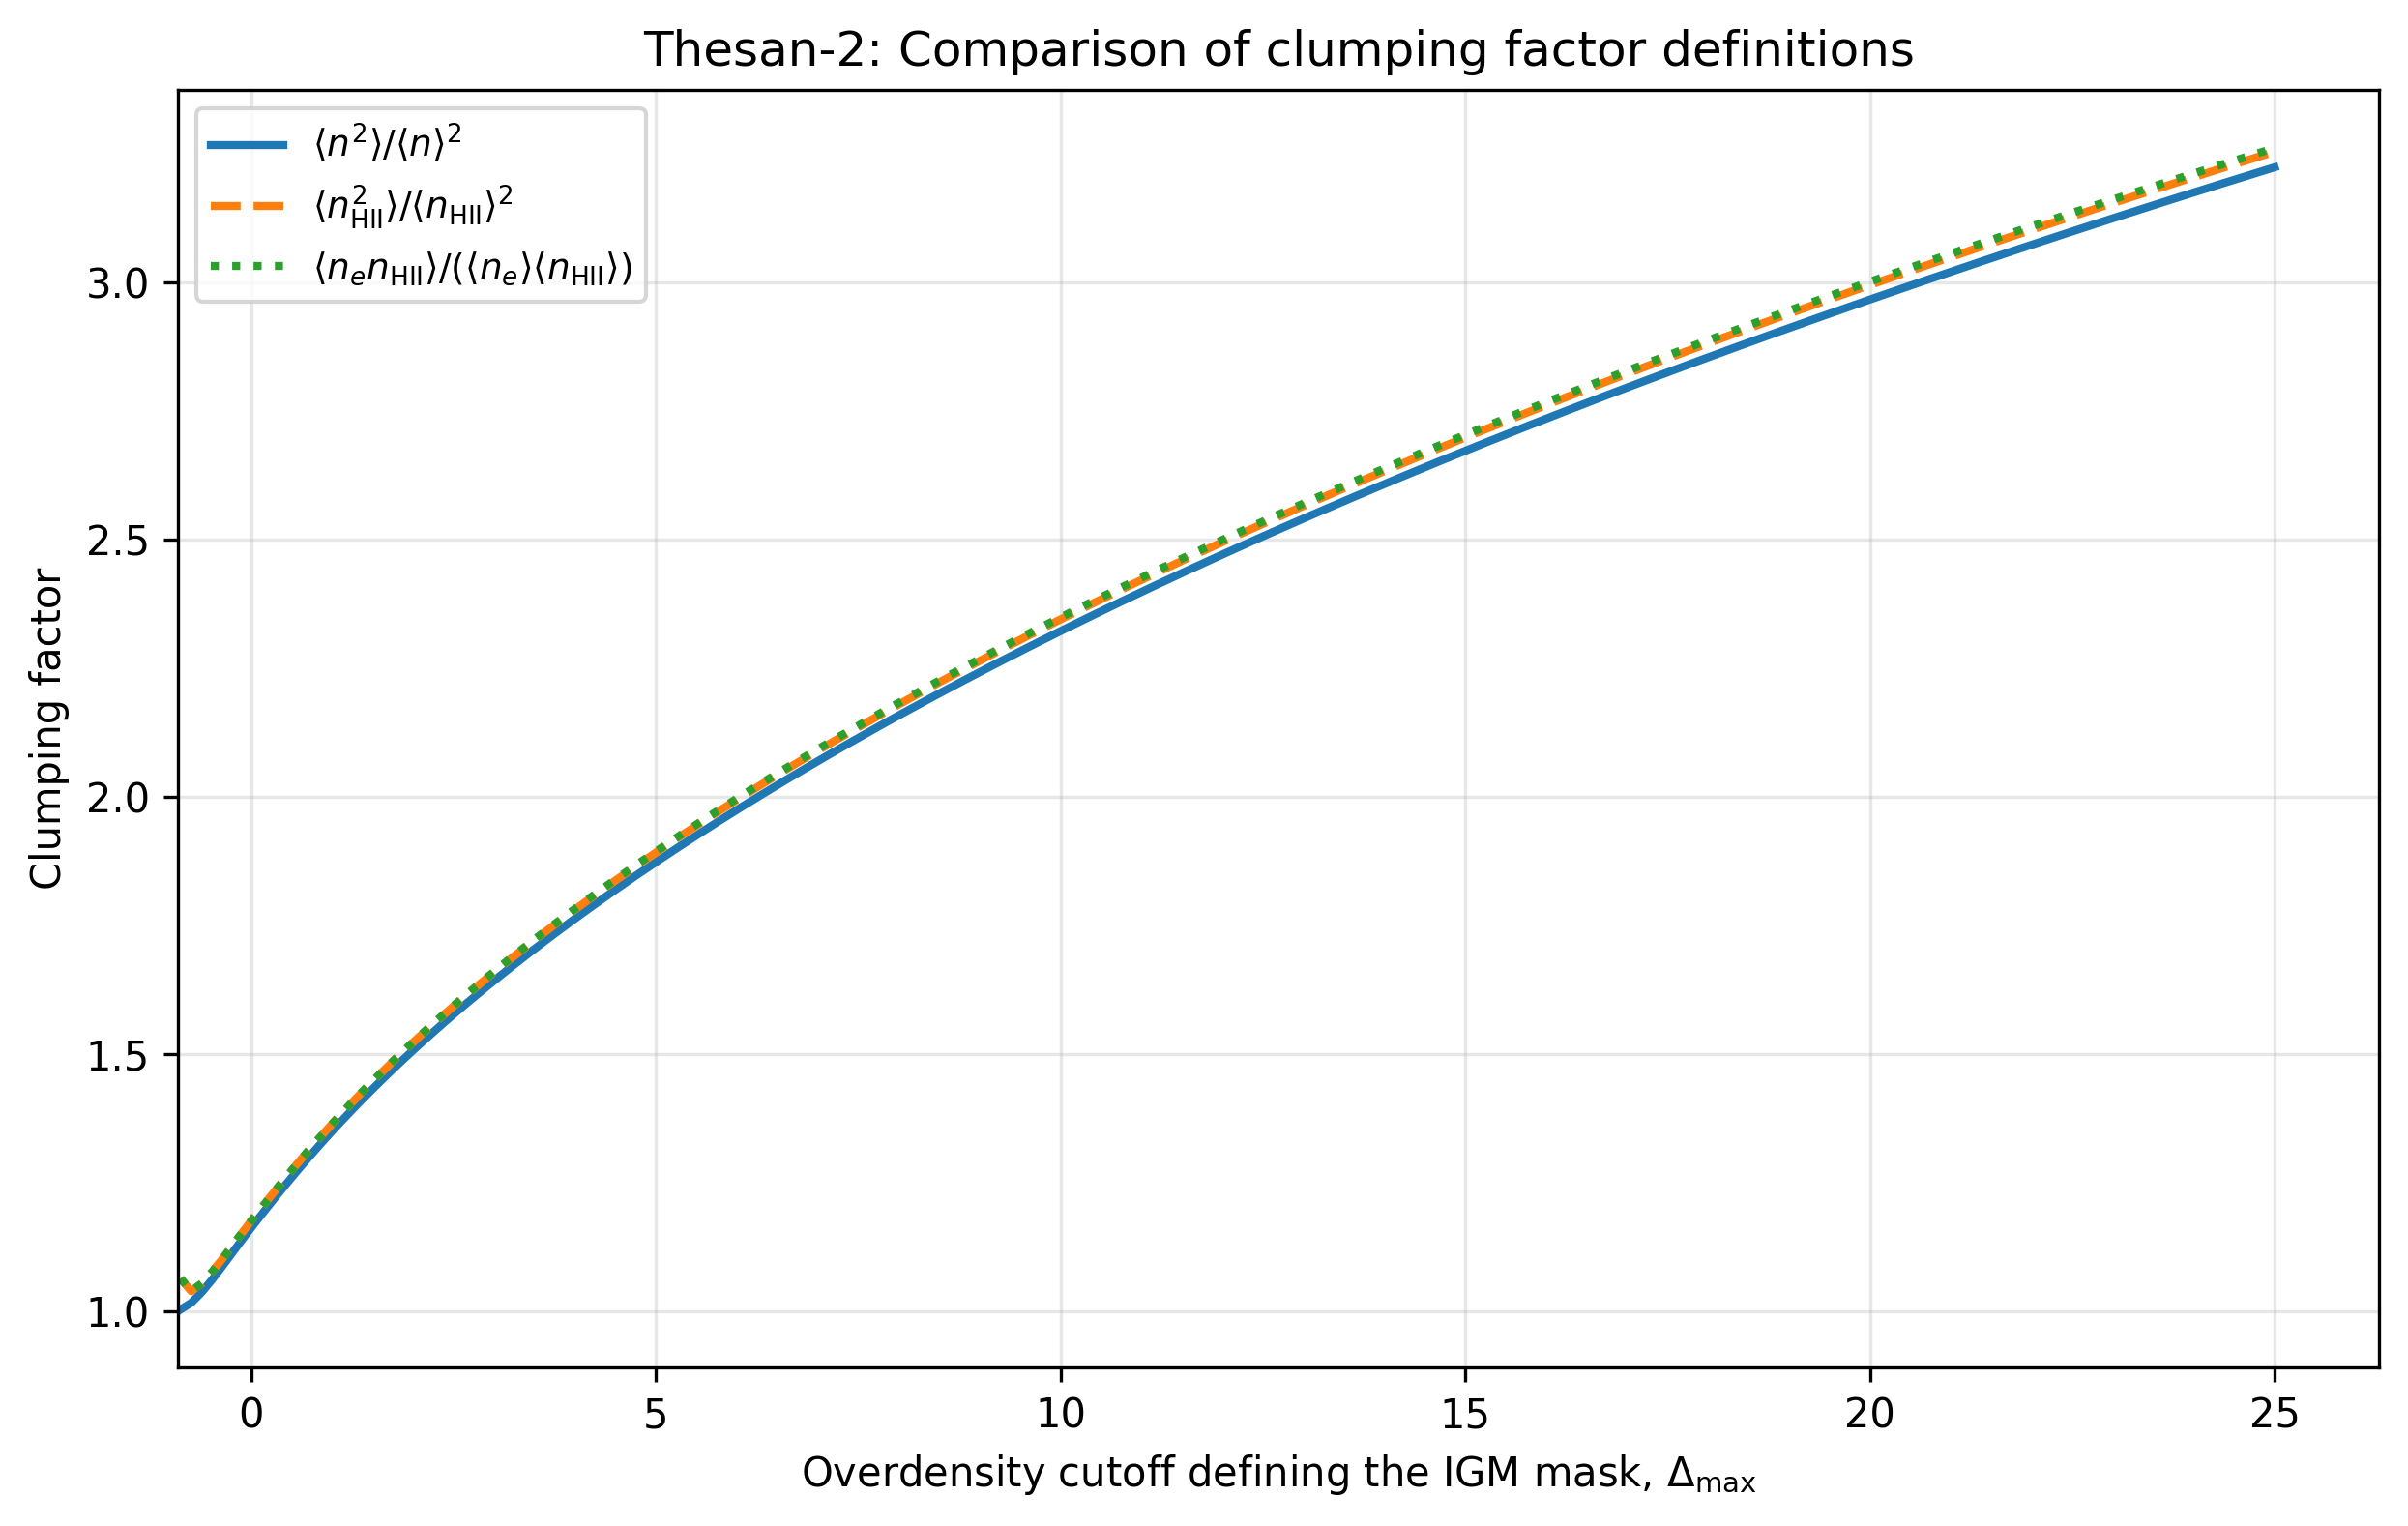
\includegraphics[width=\linewidth]{figures/thesan2_clumping_definitions_snapshot080.png}
    \end{subfigure}

    \caption{Comparison of clumping-factor definitions at snapshot 80. The upper and lower panels show THESAN-1 and THESAN-2, respectively. The curves are plotted as a function of the overdensity cutoff defining the IGM mask.}
    \label{fig:clumping-factor-definitions}
\end{figure}
 

These all behave in a very similar way, with the difference between them below $0.36\%$ for THESAN-1 and $1.16\%$ for THESAN-2 when considering the values for $\Delta_{\max} \geq 0$ to avoid the artifacts found at $\Delta_{\max} \approx -1$.

We also note that there is an almost perfect proportionality relationship between $\langle n_{HII} \rangle$ and $\langle n_e \rangle$ of about $\chi_e \approx 1.08$ which matches the value presented by Davies et al to account for the enhancement in the number of free electrons due to ionized helium. 

\begin{figure}
    \centering
    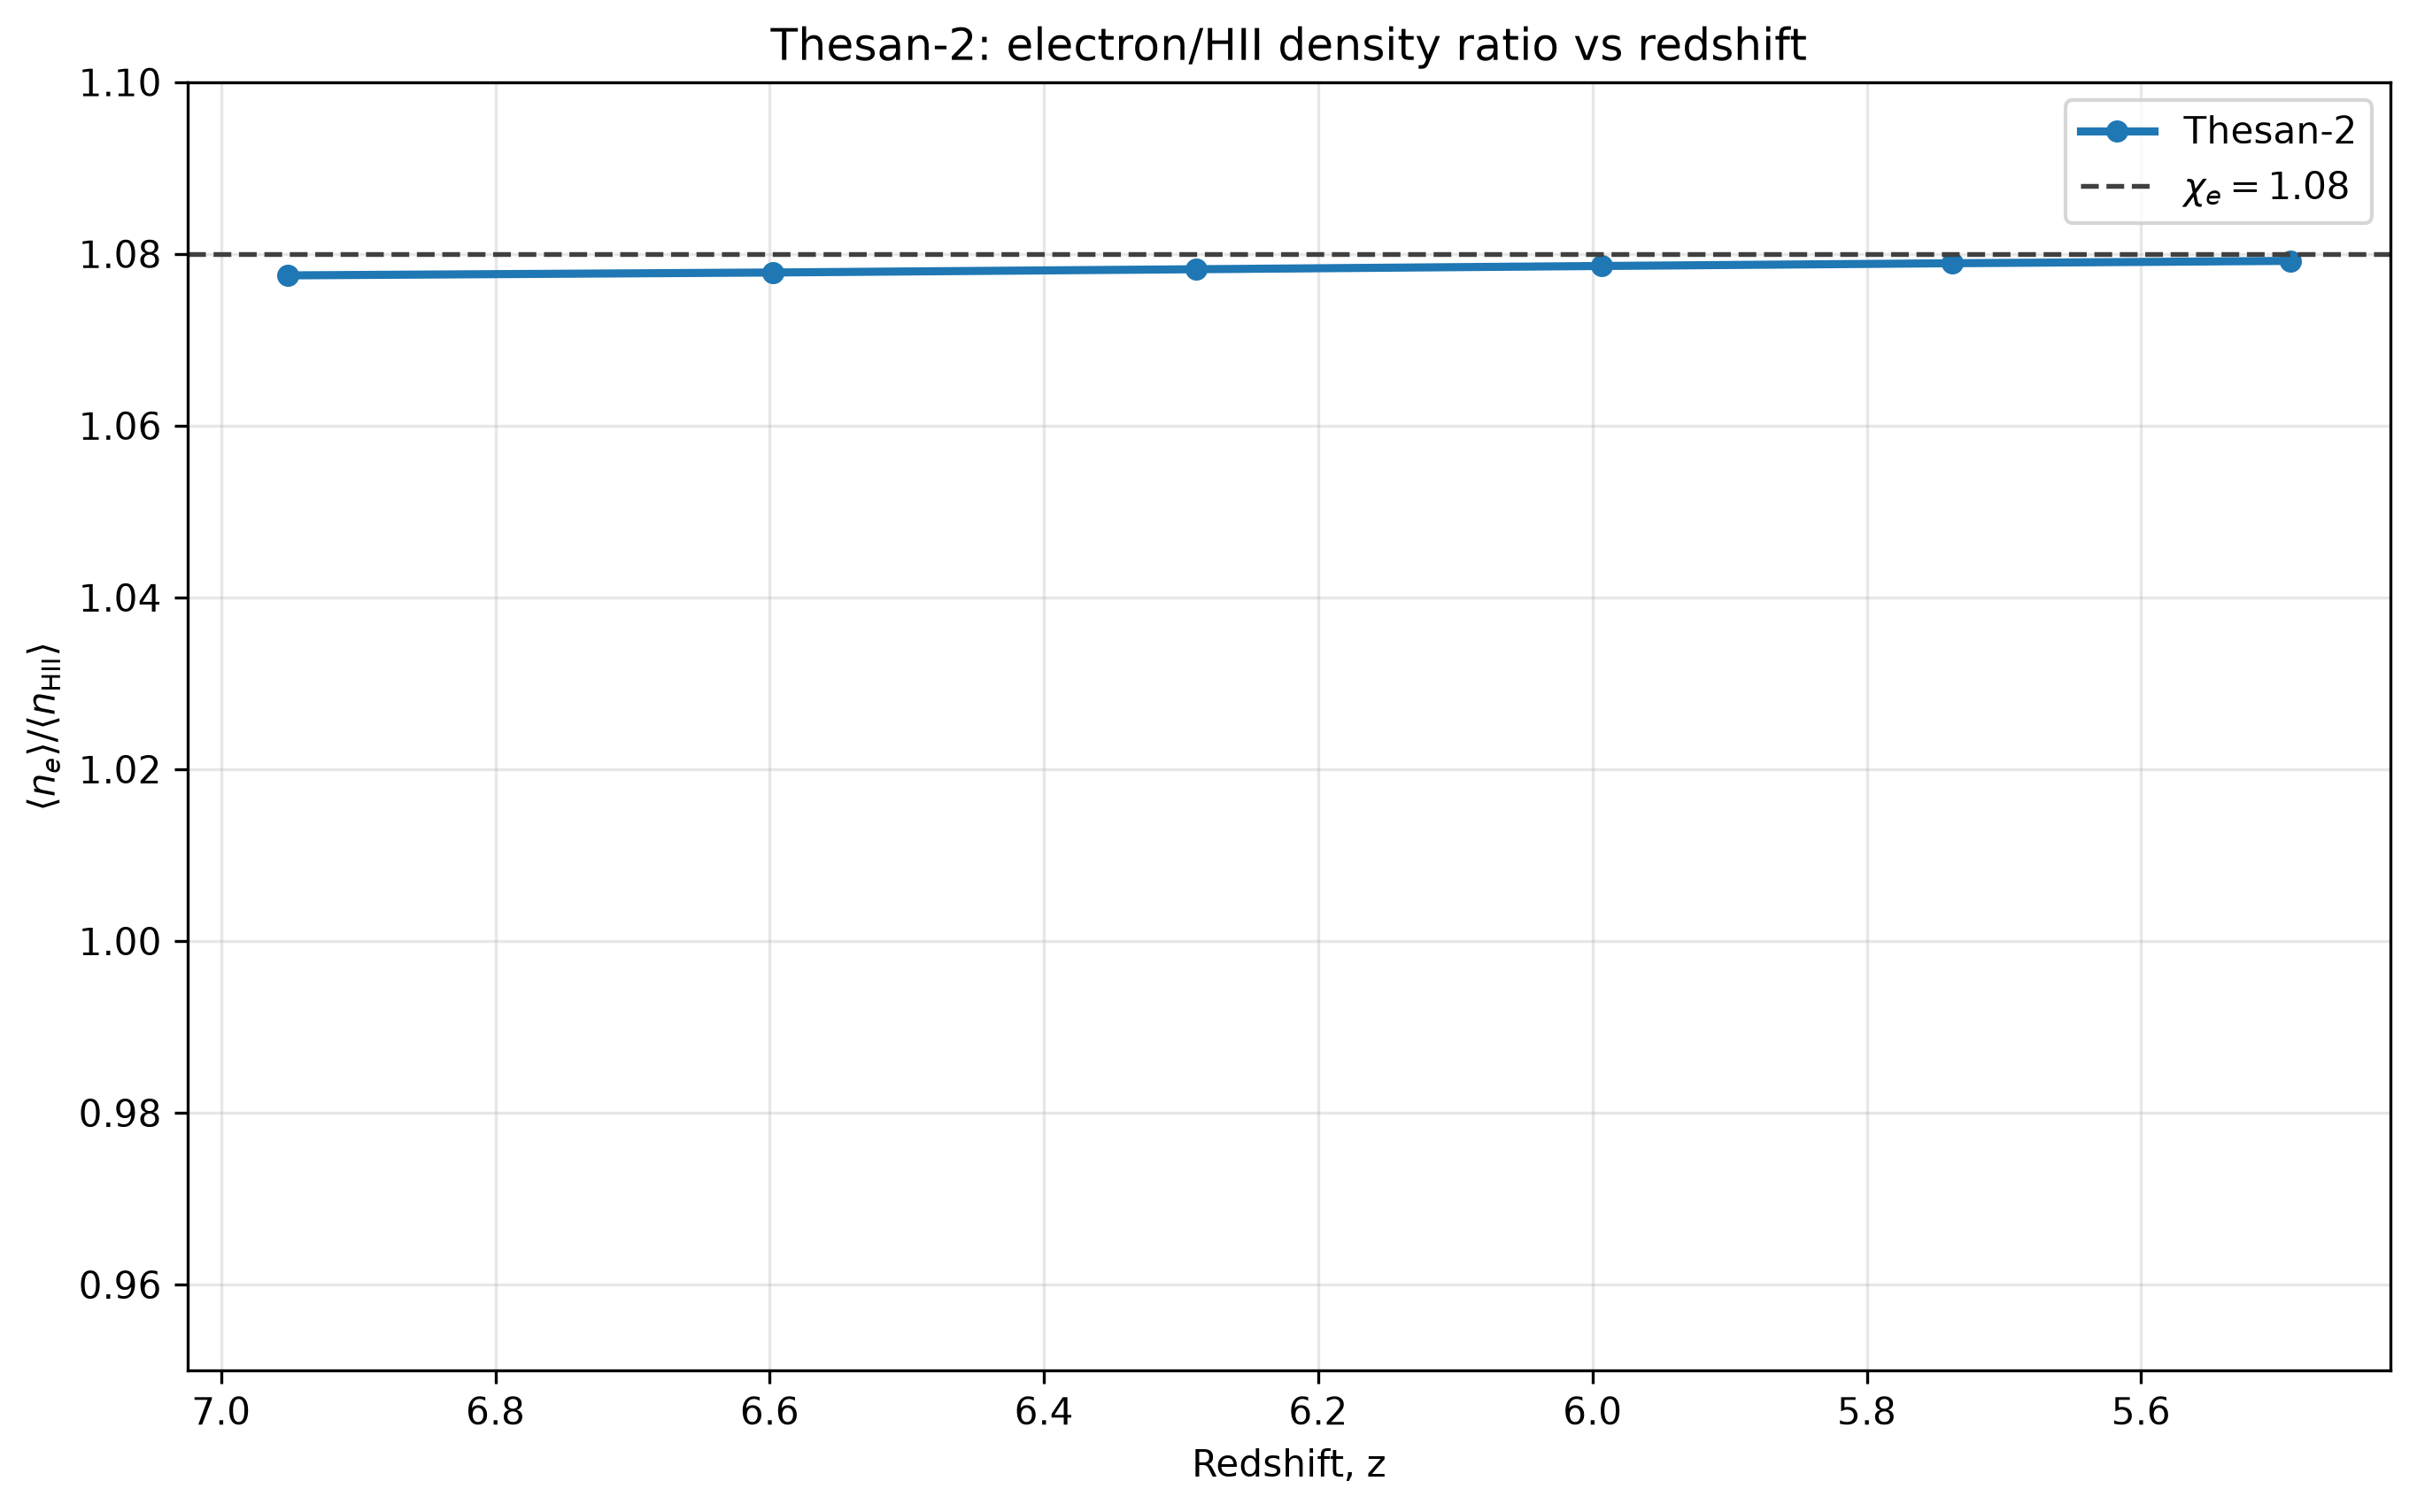
\includegraphics[width=\linewidth]{figures/thesan2_electron_density_ne_over_nHII_vs_redshift_all_gas_chi_e.png}
    \caption{Ratio of free-electron density to ionized-hydrogen density as a function of redshift for all gas in THESAN-2. The approximately constant value supports the use of $\chi_e\simeq1.08$ in the ionized gas.}
    \label{fig:electron-ratio}
\end{figure}

\section{Approximate estimator 1: ionization equilibrium}

The first approximate estimator assumes ionization equilibrium.

We make the ionization equilibrium assumption
$$\langle n_{\mathrm{H\,I}} \Gamma_{\mathrm{H\,I}} \rangle
=
\left\langle
n_e n_{\mathrm{H\,II}} \alpha_{\mathrm{H\,II}}
\right\rangle
=
C \chi_e \left(1-x_{\mathrm{H\,I}}\right)^2
n_{\mathrm{H}}^2 \alpha_{\mathrm{H\,II}}$$

which corresponds to 
$$ \langle n_{HI}\Gamma_{HI} \rangle = \langle n_e n_{\mathrm{H\,II}} \alpha_{\mathrm{H\,II}} \rangle$$

Figure~\ref{fig:ionization-equilibrium} shows that the equality is approached only after imposing a more restrictive ionization cut. This is consistent with the presence of neutral islands in the available snapshots, which are taken before the end of reionization.

\begin{figure}
    \centering
    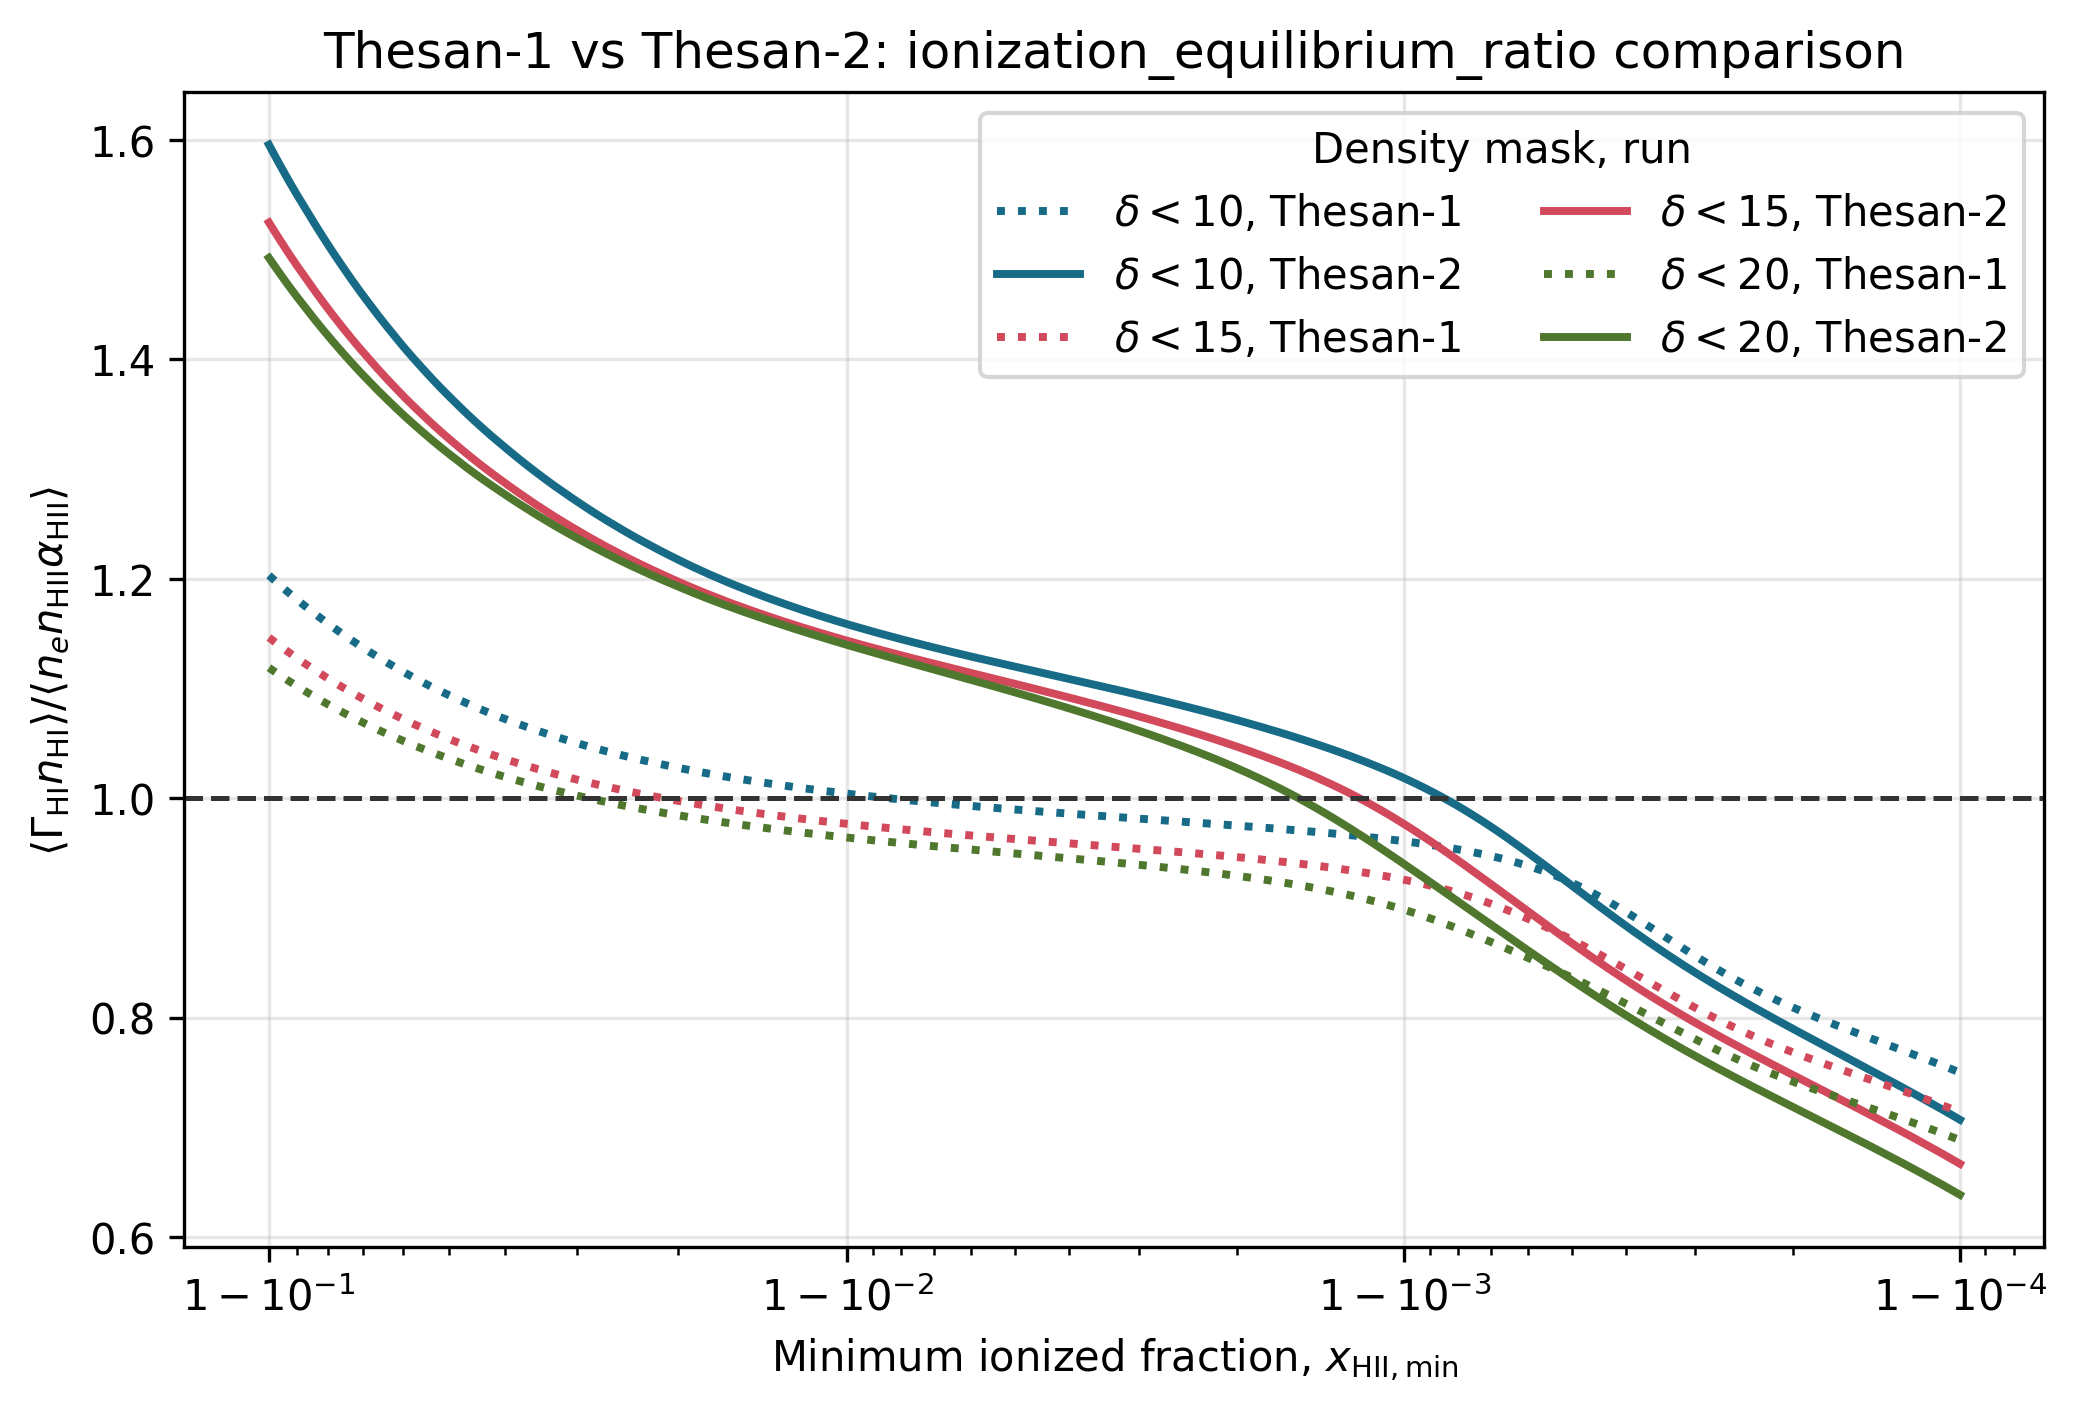
\includegraphics[width=\linewidth]{figures/thesan1_thesan2_ionization_equilibrium_ratio_vs_ionization_cut.png}
    \caption{Ratio of the photoionization and recombination rates as a function of the minimum ionized fraction used in the IGM mask. The horizontal line marks exact ionization equilibrium.}
    \label{fig:ionization-equilibrium}
\end{figure}

Davies et al. additionally approximate the mean free path by $\lambda_{\mathrm{mfp}}=(n_{\mathrm{H\,I}}\sigma_{\mathrm{H\,I}})^{-1}$. Figure~\ref{fig:meanfreepath-sigma} shows that this approximation introduces a systematic bias in the region where ionization equilibrium is closest to being satisfied. Thus, the two assumptions cannot generally be imposed simultaneously for the masks considered here.
\begin{figure}
    \centering
    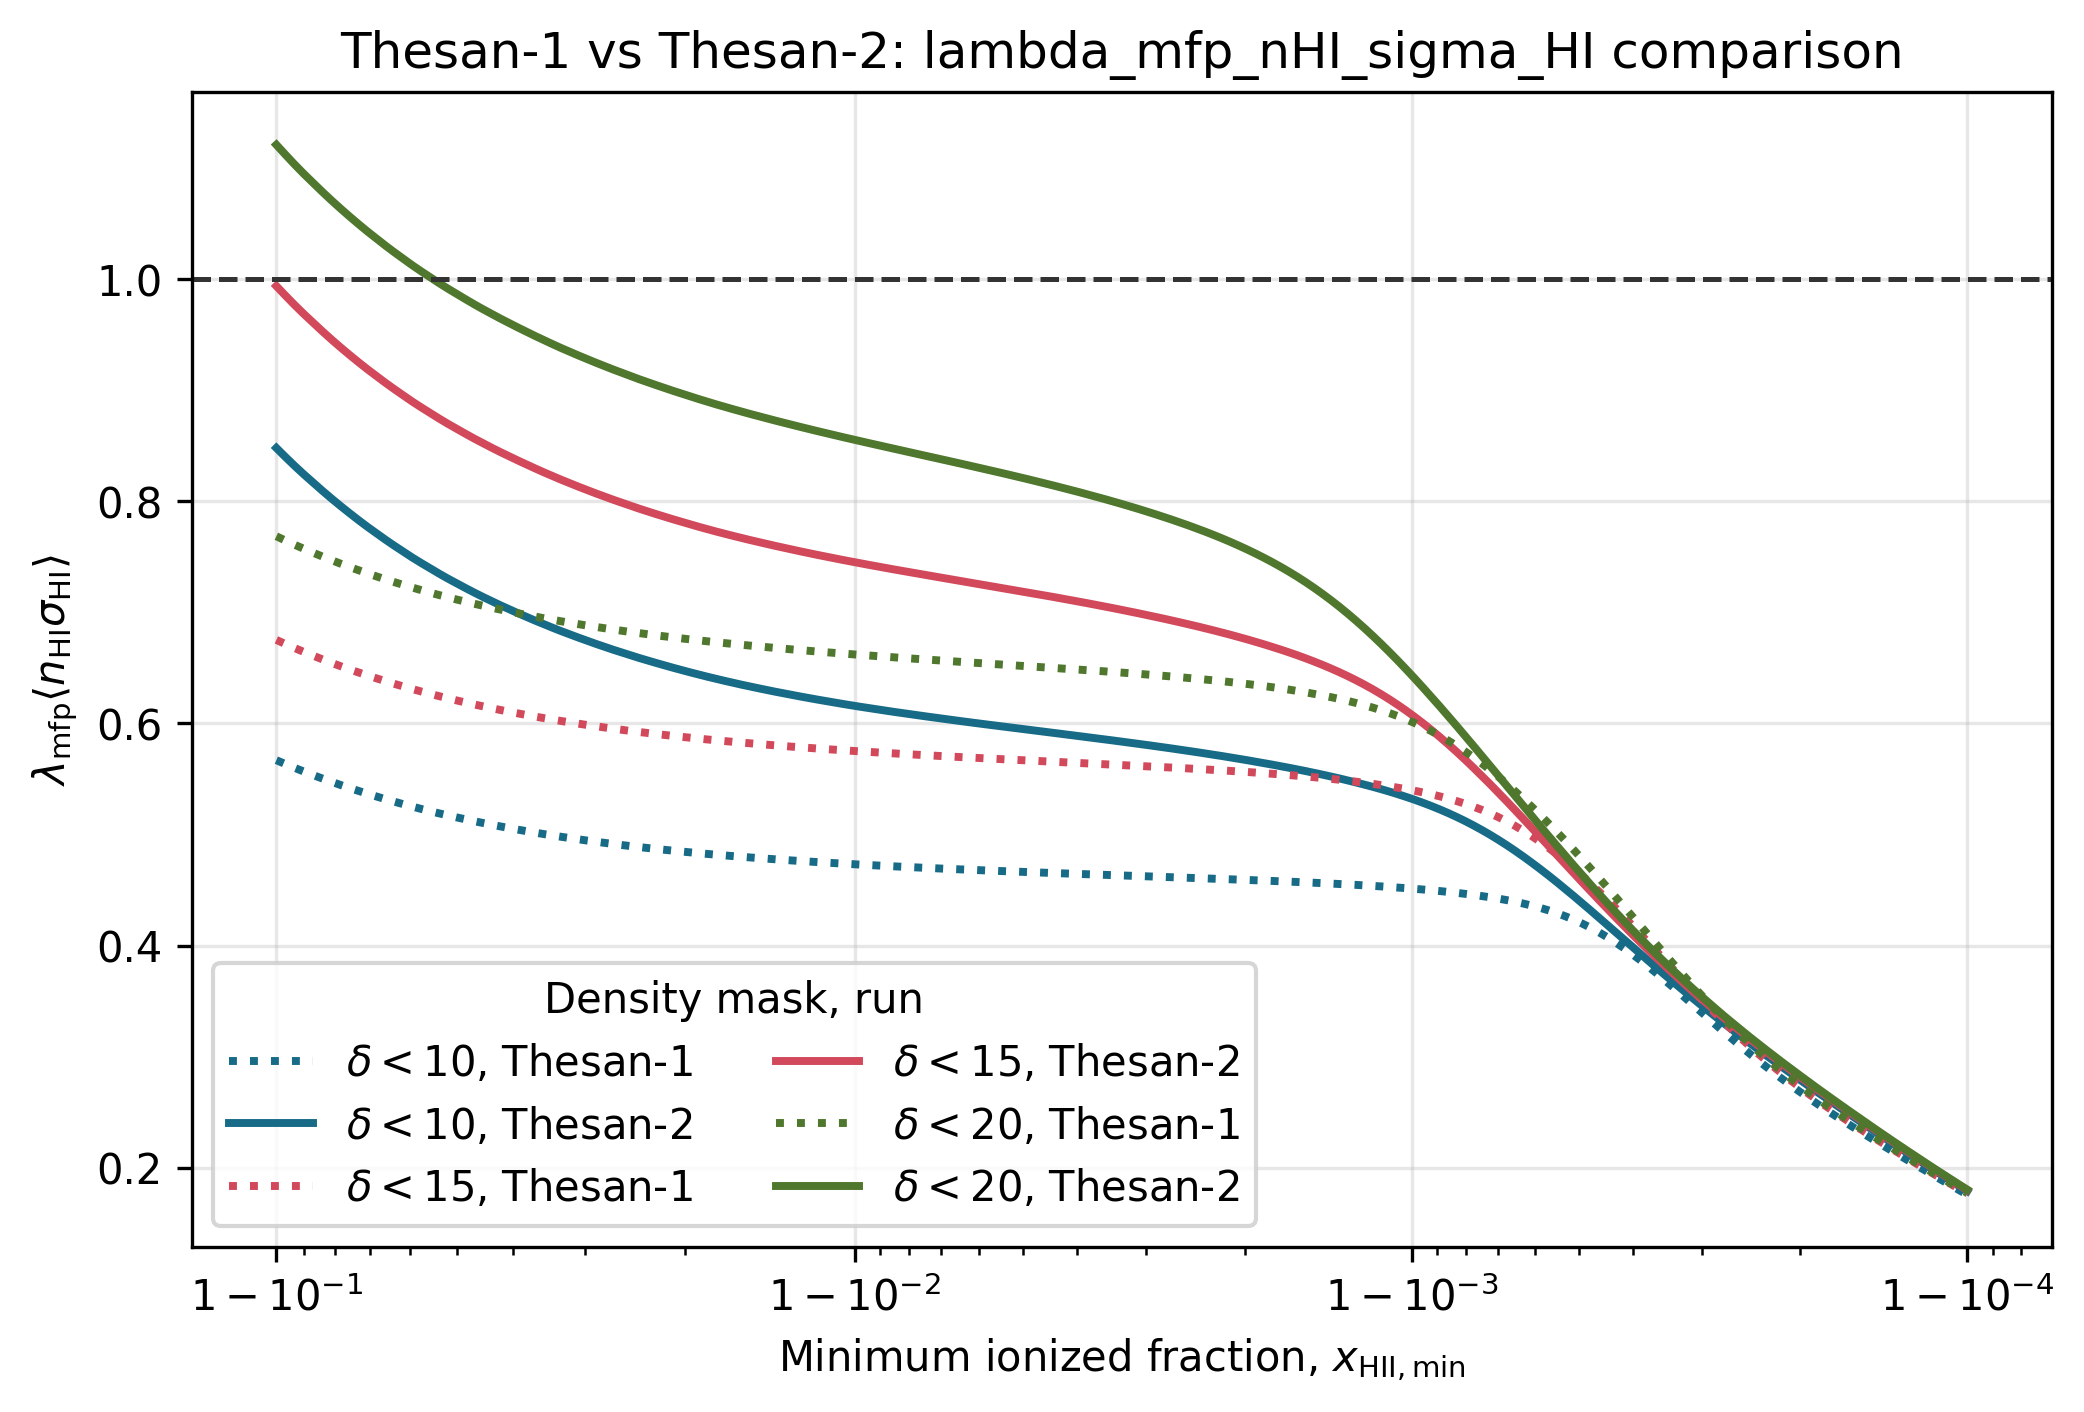
\includegraphics[width=\linewidth]{figures/thesan1_thesan2_lambda_mfp_nHI_sigma_HI_vs_ionization_cut.png}
    \caption{Ratio of the line-of-sight mean free path to the estimate $(n_{\mathrm{H\,I}}\sigma_{\mathrm{H\,I}})^{-1}$ as a function of the ionization cut. The horizontal line marks equality.}
    \label{fig:meanfreepath-sigma}
\end{figure}


Combining these assumptions gives the first approximate estimator,

$$C = \frac{ \Gamma_{\mathrm{H\,I}}}
{\lambda_{\mathrm{mfp}} \sigma_{\mathrm{H\,I}} \chi_e \left(1-x_{\mathrm{H\,I}}\right)^2 n_{\mathrm{H}}^2 \alpha_{\mathrm{H\,II}}}$$



\section{Approximate estimator 2: photon-density closure}
A second estimator defines an effective photon interaction rate by $\Gamma_{\gamma}=c/\lambda_{\mathrm{mfp}}$. The corresponding photoionization rate per unit volume is then assumed to balance the recombination rate:
$$\frac{n_{\gamma} c}{\lambda_{\mathrm{mfp}}}  = \langle n_e n_{\mathrm{H\,II}} \alpha_{\mathrm{H\,II}} \rangle .$$

The THESAN simulations use a reduced speed of light. We therefore use
the corresponding reduced value of $c$ in this closure relation. Even
after this correction, the relation is not satisfied for the masks
examined here. The resulting discrepancy is shown in
Fig.~\ref{fig:photon-density} and introduces an additional
multiplicative factor in the inferred clumping factor.

\begin{figure}
    \centering
    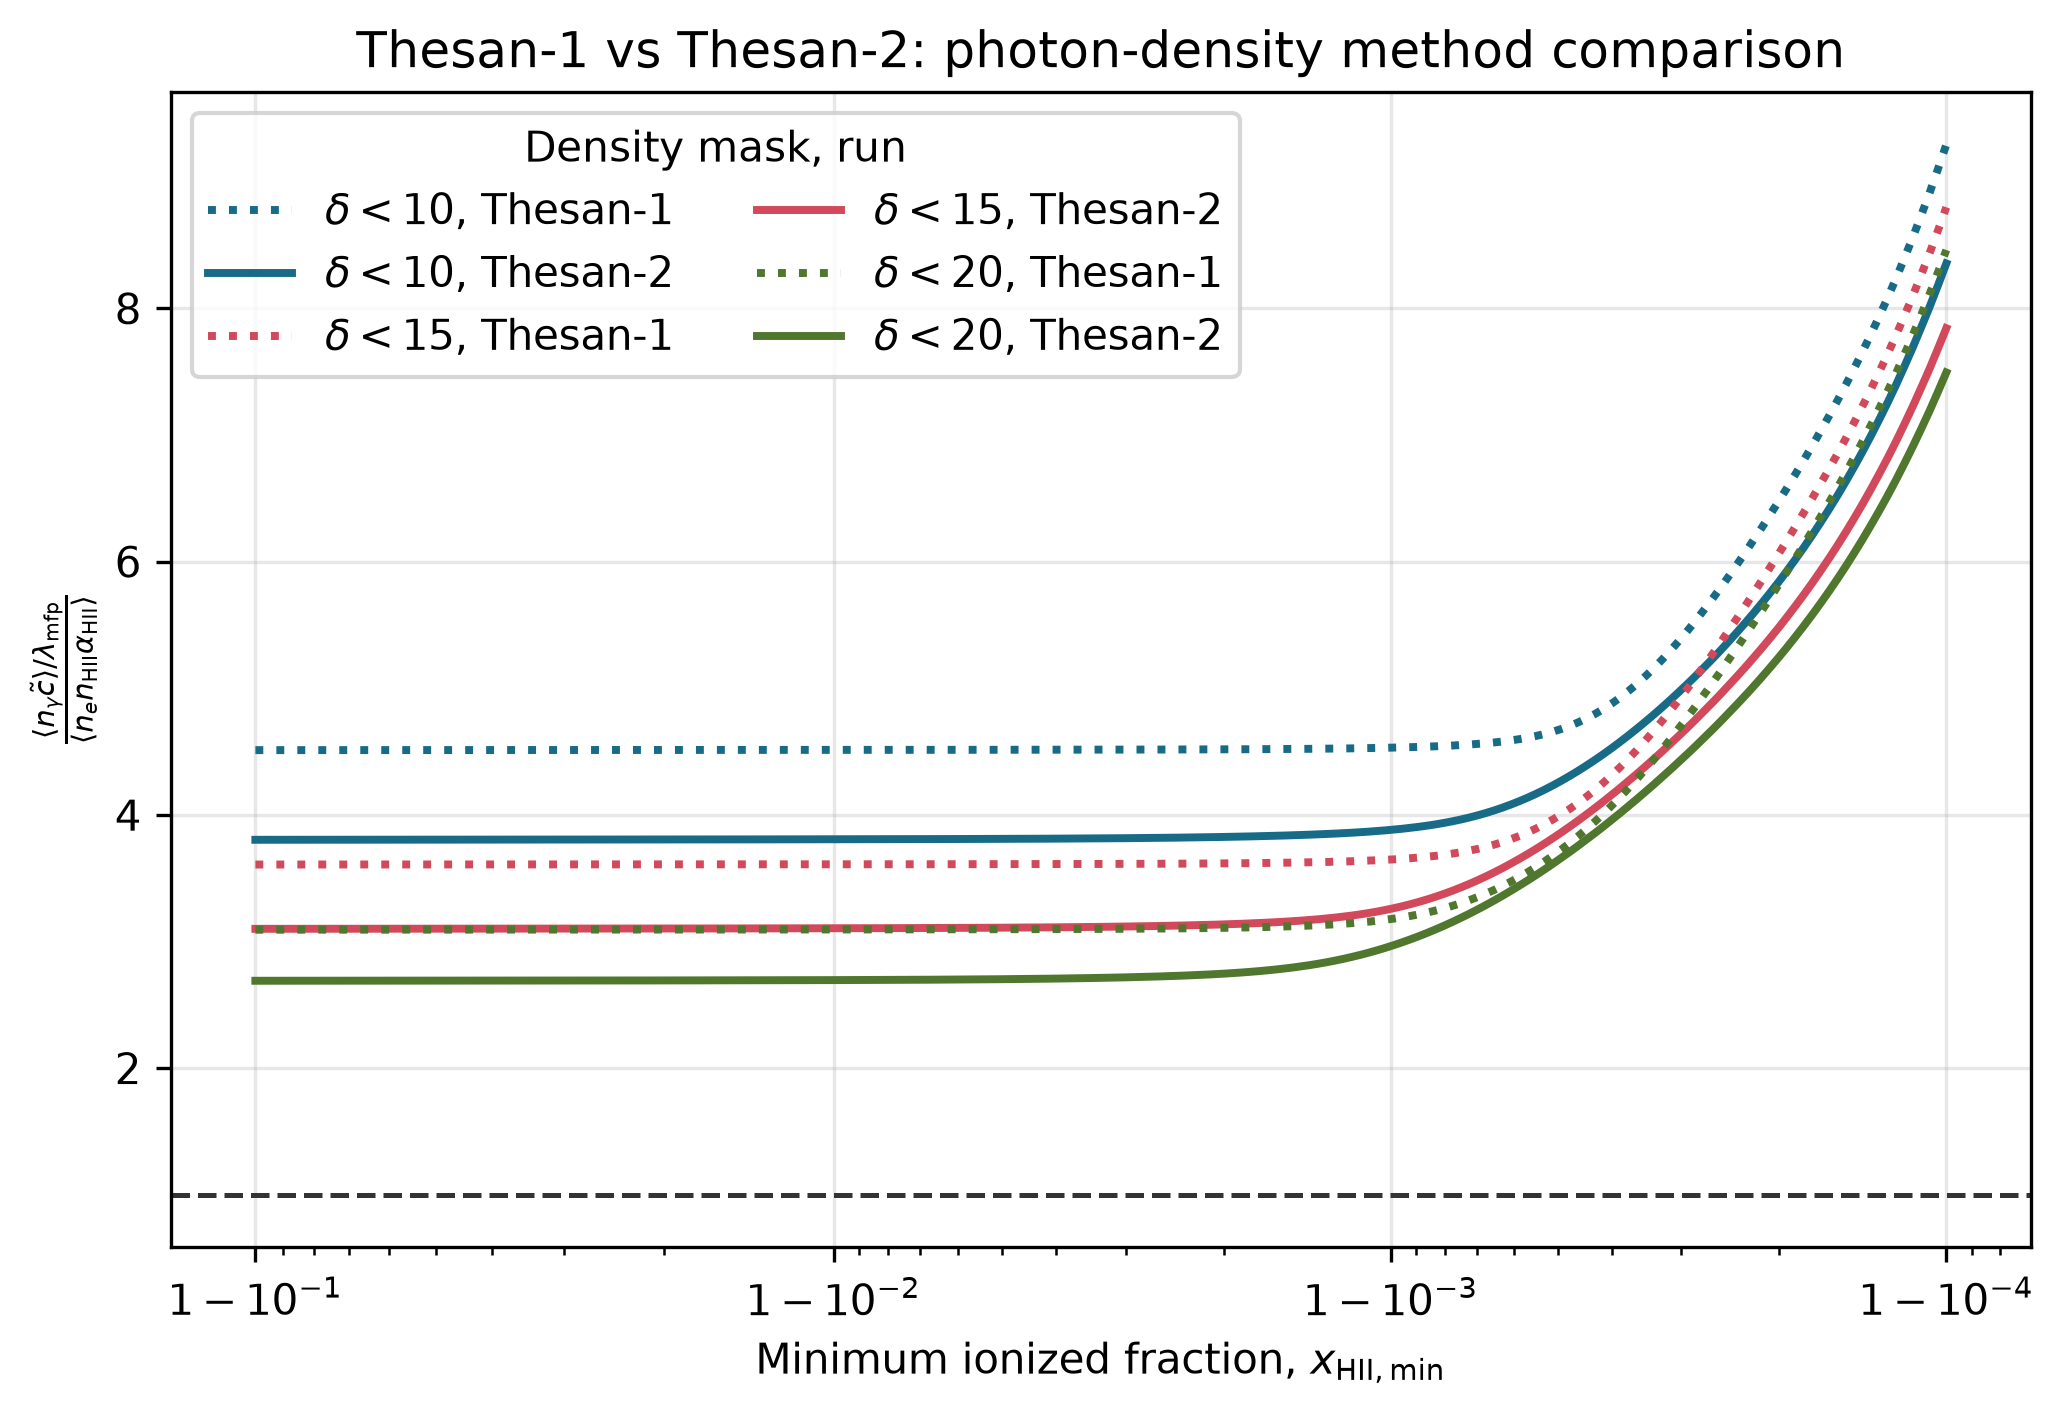
\includegraphics[width=\linewidth]{../results/analysis/clumping/thesan/combined-snapshots/forest/davies10k/thesan1_thesan2_photon_density_reduced_c_over_standard_vs_ionization_cut.png}
    \caption{Ratio between the photon-density closure estimate and the
    standard recombination rate, including the reduced speed of light,
    as a function of the minimum ionized fraction defining the IGM
    mask. The horizontal line marks agreement between the two rates.}
    \label{fig:photon-density}
\end{figure}

The resulting estimator is
$$C = \frac{ n_{\gamma} c}
{\lambda_{\mathrm{mfp}}  \chi_e \left(1-x_{\mathrm{H\,I}}\right)^2 n_{\mathrm{H}}^2 \alpha_{\mathrm{H\,II}}}.$$

\section{Comparison of clumping-factor estimators}

We have tested the assumptions entering the approximate estimators
individually. We now compare the resulting clumping factors with the
direct calculation for the THESAN simulations. The comparison is shown
in Fig.~\ref{fig:clumpingfactors} for several choices of the minimum
ionized fraction defining the IGM mask.

The direct calculation provides the reference result. Depending on the
overdensity threshold, its clumping factor is typically between
approximately 2 and 4. The estimator based on ionization equilibrium
gives a slightly larger value, with its closest agreement with the
reference result occurring for
$10^{-3}\lesssim x_{\mathrm{H\,II,min}}\lesssim10^{-2}$.

Including the additional approximation
$\lambda_{\mathrm{mfp}}=(n_{\mathrm{H\,I}}\sigma_{\mathrm{H\,I}})^{-1}$
increases the discrepancy. In the range where ionization equilibrium is
approximately satisfied, this estimator introduces a correction of up
to a factor of approximately 2.5 relative to the direct calculation.

The photon-density estimator gives the largest clumping factors. After
accounting for the reduced speed of light used in the THESAN
simulations, it still exceeds the direct estimate by up to a factor of
approximately 5 for the masks considered here.

These results show that the approximate estimators are sensitive not
only to the definition of the IGM but also to the assumptions used to
relate the mean free path, photoionization rate, and recombination rate.
No single approximate estimator reproduces the direct clumping factor
over the full range of masks examined here. The ionization-equilibrium
estimator performs best in the restricted regime where the equilibrium
assumption is approximately valid, whereas the additional mean-free-path
and photon-density closures introduce substantial systematic biases.

\begin{figure*}[t]
    \centering
    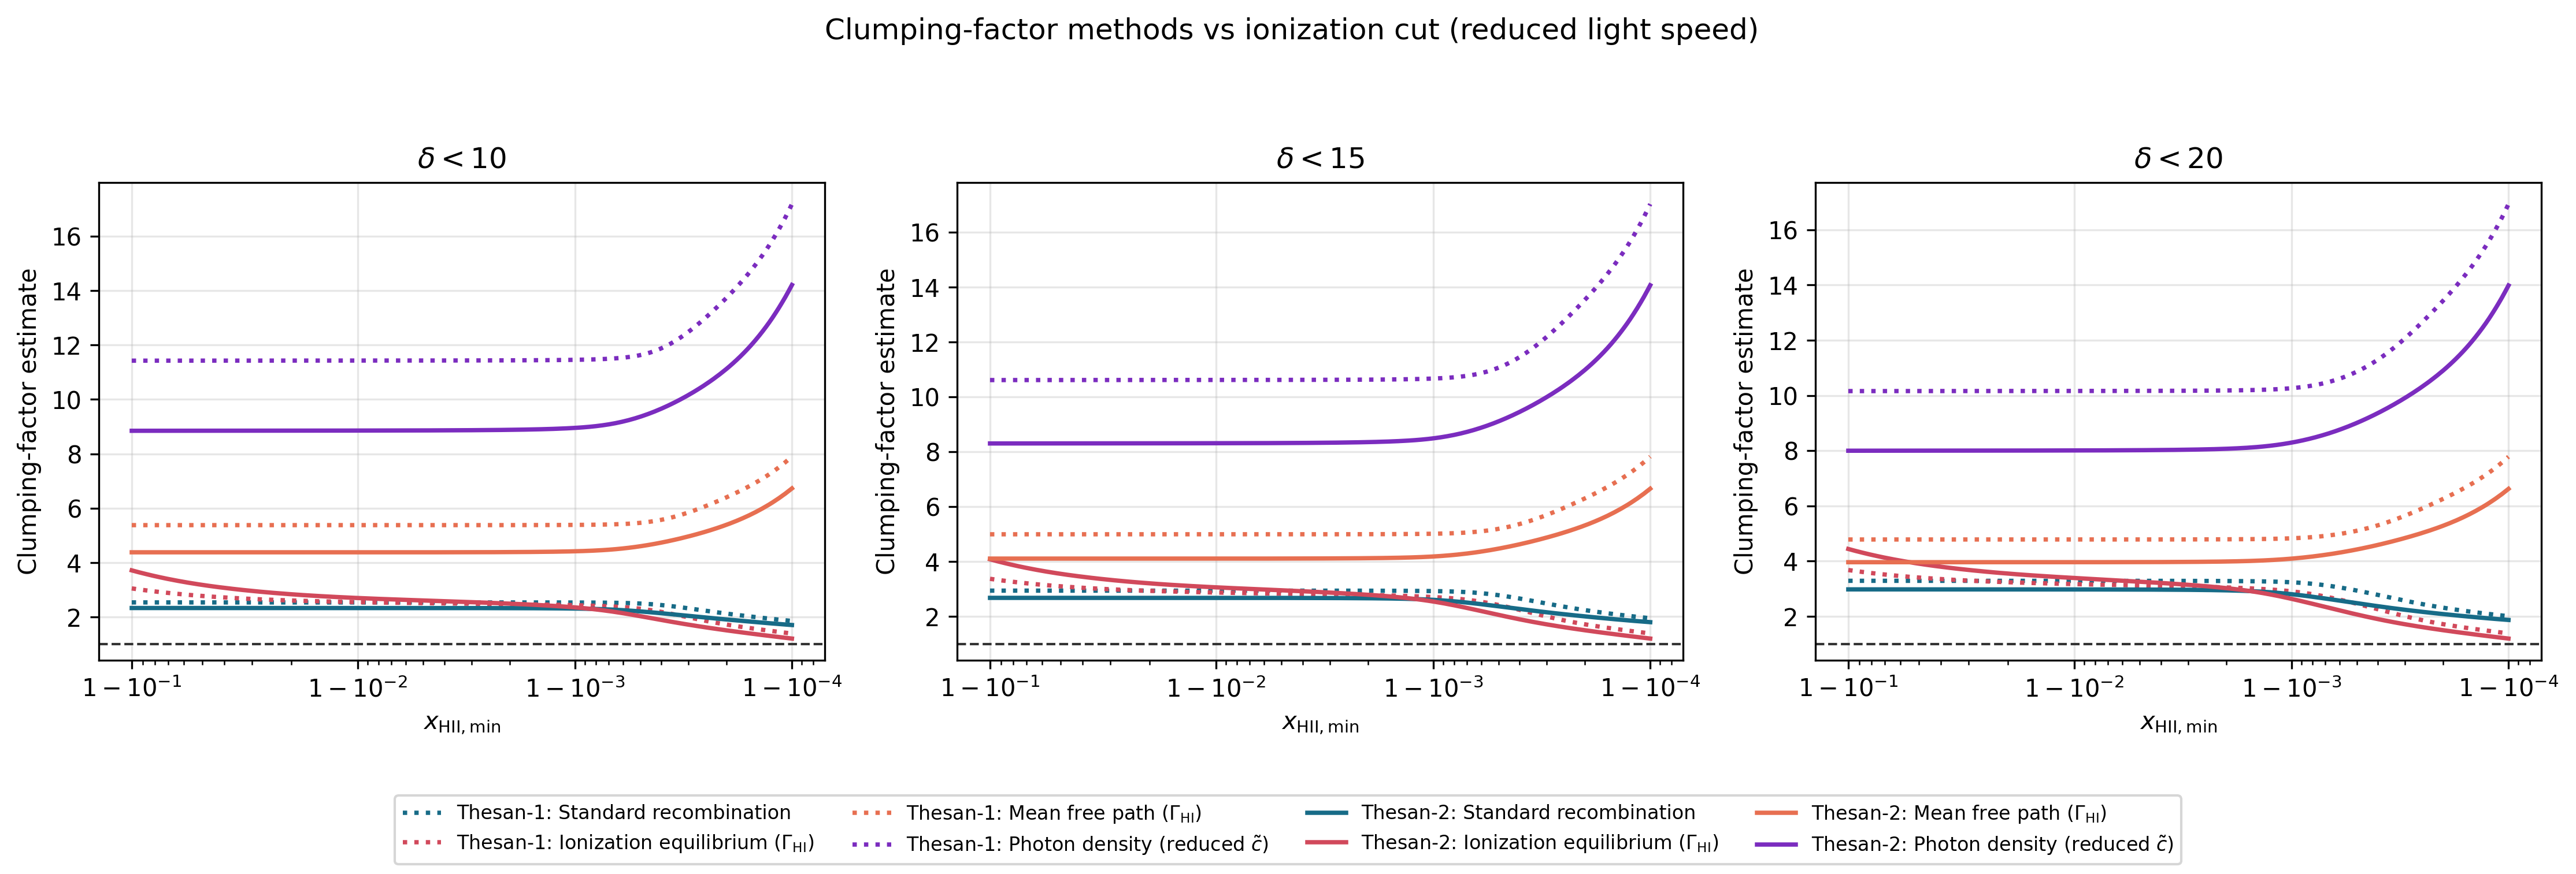
\includegraphics[width=0.96\textwidth]{../results/analysis/clumping/thesan/combined-snapshots/forest/davies10k/thesan1_thesan2_clumping_methods_reduced_c_vs_ionization_cut.png}
    \caption{Comparison of the direct and approximate clumping-factor
    estimators as a function of the minimum ionized fraction defining
    the IGM mask. The three panels correspond to overdensity thresholds
    $\Delta<10$, $\Delta<15$, and $\Delta<20$, respectively. The direct
    estimate is compared with the ionization-equilibrium, mean-free-path,
    and photon-density estimators. The photon-density estimator uses the
    reduced speed of light adopted in the THESAN simulations.}
    \label{fig:clumpingfactors}
\end{figure*}


\bibliography{apssamp}
\end{document}
%
% ****** End of file apssamp.tex ******
